\chapter{Zadania dodatkowe}
	\label{ch:dod}
	\section{PID}
		\label{sec:PID}
		Algorytm PID oblicze przyszłe sterowanie na podstawie wartości, pochodnej i całki uchybu w odpowiednich proporcjach. Popularną sposobem strojenia tego regulatora jest metoda Zieglera-Nicholsa, która polega na doprowadzenie obiektu na granice stabilności przy wyłączonych członach I oraz D, zmierzenia okresu drgań a następnie podstawieniu odpowiednich wartości do wzoru. W przypadku obiektu z zadania obiekt był na granicy stabilności (w we wszystkich zadanych przez nas punktach pracy) przy $K_p=4$, co można zaobserwować na rys. \ref{fig:PID0}.
		
		\begin{figure}[h!]
			\centering
			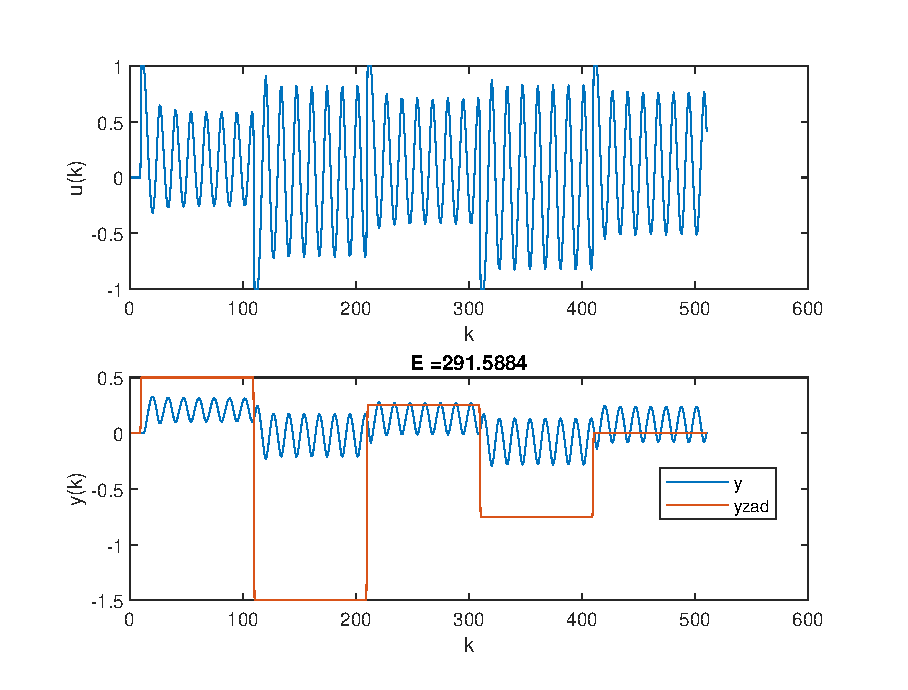
\includegraphics[width=\linewidth]{img/strojeniePID_Kp_4_Ti_duzo_Td_0.eps}
			\caption{Działanie regulatora PID z nastawami Kp = 4, Ti = Inf, Td = 0}
			\label{fig:PID0}
		\end{figure}
		
		Następnie, po podstawieniu zmierzonych wartości (okres drgań $T_u=13$) otrzymaliśmy przebieg przedstawiony na rys. \ref{fig:PID1}.
		Widać, że regulator próbuje naśladować przebieg wartości zadanej, i robi to nie najgorzej (mimo bardzo ostrego sterowania), lecz dla niektórych punktów pracy pojawiają się niegasnące oscylacje.
		
		\begin{figure}[h!]
			\centering
			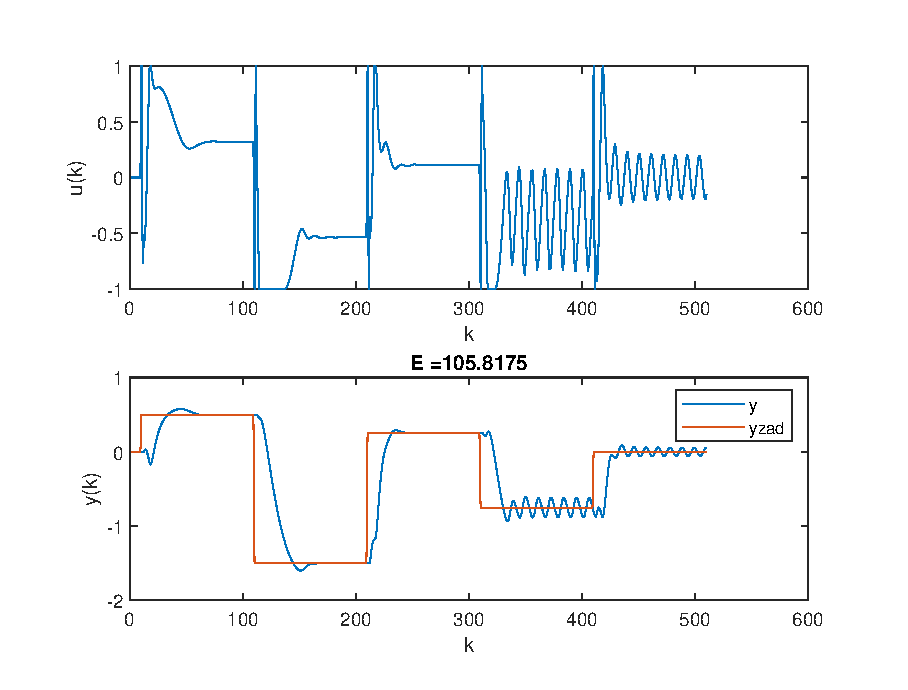
\includegraphics[width=\linewidth]{img/strojeniePID_Ziegler_Nichols.eps}
			\caption{Działanie regulatora PID z nastawami Kp = 2.4, Ti = 6.5, Td = 1.625}
			\label{fig:PID1}
		\end{figure}
		
		
	\section{NO}
		\label{sec:NO}
		Algorytm NO, tym różni się od algorytmu NPL, że do wyznaczania predykcji wyjścia stosuje się model nieliniowy. Oznacza to, że nie można wyznaczyć przyszłych sterowań analitycznie. Posługując się wskaznikiem jakości
		\begin{equation}
		\begin{tabular}{l}
		$J(k) = \sum\limits_{p=1}^{N}(y^{zad}(k)-\hat{y}(k+p|k))^2+\lambda\sum\limits_{p=0}^{N_u}(\Delta u(k+p|k))^2$
		\end{tabular}
		\label{eq:wsk_jakosc}
		\end{equation}
		wyznacza się takie sterowania dla których jest on najmniejszy.
		Wyliczyjąć predykcje wyjścia jako
		\begin{equation}
		\begin{tabular}{l}
		$\hat{y}(k+p|k)=w20 + w2*tanh(w10+w1*x(k+p|k))+dk$
		\end{tabular}
		\label{eq:NO_wyjscie}
		\end{equation}
		gdzie
		\begin{equation}
		\begin{tabular}{l}
		$x(k+p|k)=\begin{bmatrix}u(k-3+p)\\u(k-4+p)\\y(k-1+p)\\y(k-2+p)\end{bmatrix}$
		\end{tabular}
		\label{eq:NO_wesn}
		\end{equation}
		We wzorze tym, podobnie jak w równaniu \ref{eq:NPL_y0} i \ref{eq:GPC_y0} dla $y(n>k)=\hat{y}(n|k)$. Dodatkowo dochodzi jeszcze $u(n \geqslant k+N_u)=u(k+N_u-1)$. Mojąc wyznaczone wszystkie wartości można obliczyć zadanie optymalizacji. Wyniki działania algorytmu NO przedstawione są na rysunku \ref{fig:NO}.
		\begin{figure}[h!]
			\centering
			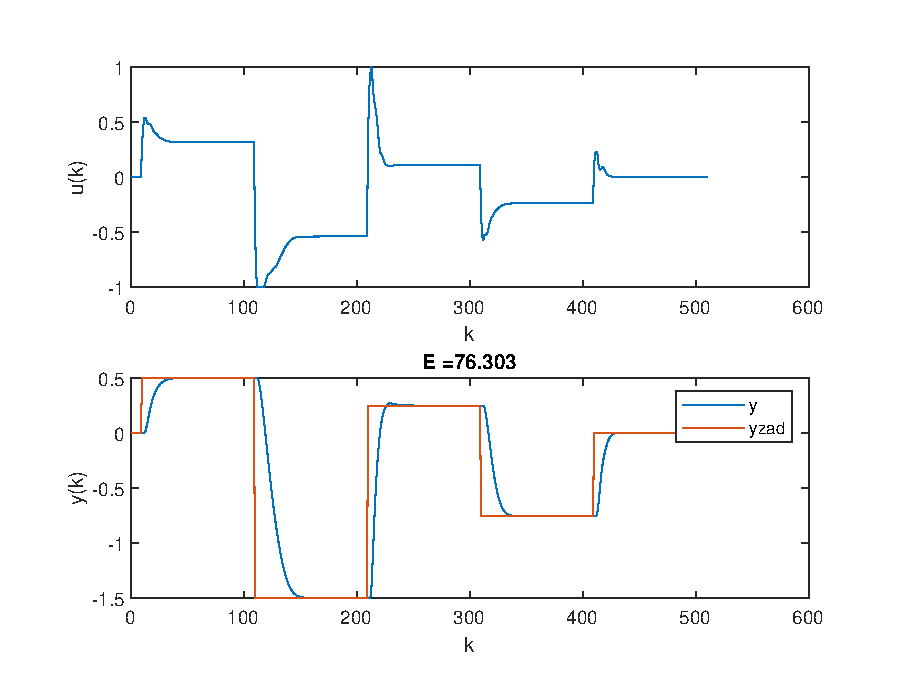
\includegraphics[width=\linewidth]{img/NO.eps}
			\caption{Działanie regulatora NO z nastawami N=20, Nu=2, $\lambda$=2}
			\label{fig:NO}
		\end{figure}
		Jak widać zarówno wyjscie obiektu jak i sterowania wyglądają swiętnie. Niestety dużą wadą algorytmu NO jest, fakt że w każdym kroku algorytmu należy rozwiązać zadanie nieliniowej optymalizacji, co w przypadku obiektów o dłuższych horyzontach predykcji potrafi prowadzić do bardzo długiego czasu wyznaczania sterowań.